\chapter{Experimental Results}
\section{Experimental Methodology}

%Add the introduction sentence, we compare so-and-so with standard MAUT
We use two standard datasets in our experiments - \textbf{Camera} and \textbf{PC}.
Both the datasets are available for download at \url{http://www.cs.ucd.ie/staff/lmcginty/PCdataset.zip}.
Cases with missing values have been removed from the dataset.
The Camera dataset contains 173 cameras with 10 attributes and the PC dataset contains 120 PCs with 8 attributes.
A typical PC in the PC dataset is shown in Table \ref{tab:pc} and a typical camera is shown in Table \ref{tab:camera}.


\begin{table}
\caption{A typical PC in the PC dataset}
\centering
\renewcommand{\arraystretch}{1.2}
\label{tab:pc}

\begin{tabular}{|l|l|}
\hline
Manufacturer & Apple \\
\hline
Processor Type & PowerPC G3 \\
\hline
Processor Speed(MHz) & 600 \\
\hline
Monitor (Inches) & 15 \\
\hline
Type & Laptop \\ 
\hline
RAM (MB) & 512 \\
\hline
Drive Capacity(GB) & 40 \\
\hline
Price (\$) & 986\\
\hline
\end{tabular}
\end{table}

\begin{table}
\caption{A typical camera in the Camera dataset}
\centering
\renewcommand{\arraystretch}{1.2}
\label{tab:camera}

\begin{tabular}{|l|l|}
\hline
Manufacturer & Sony \\
\hline
Model & DSC-T11 \\
\hline
Price(\$) & 383\\
\hline
Format & Ultra-compact\\
\hline
Resolution (MP)  &5\\
\hline
Optical Zoom (X) &3 \\
\hline
Digital Zoom (X) &4\\
\hline
Weight (grams) &230\\
\hline
Storage Type & Memory Stick\\
\hline
Storage Included (MB)& 32\\
\hline
\end{tabular}
\end{table}

To evaluate the algorithms in offline setting, we simulate an artificial user who interacts with the recommender system.
We perform the evaluation of our algorithms in two scenarios described in Section \ref{sec:focus} and \ref{sec:noisy}, where the artifical user interacts with the system in two different ways.
The complete implementation for all the improvements described in Sections \ref{sec:div} to \ref{sec:additive} is available at \url{https://github.com/abharath27/MAUTNew.git}.

\section{Highly Focused Recommendation Framework}
Evaluation in Highly Focused Recommendation Framework is the same way of evaluation described in Section \ref{sec:offline}.
In this scenario we assume that the user is relatively sure of his preferences and hence chooses the critique string that is maximally compatible with the target product in each cycle.
The notion of selecting the most compatible critique string is shown in Figure \ref{fig:focus}

%This will help  us to illustrate the noisy framework better.

\begin{figure}
  \centering
  \captionsetup{justification=centering}
    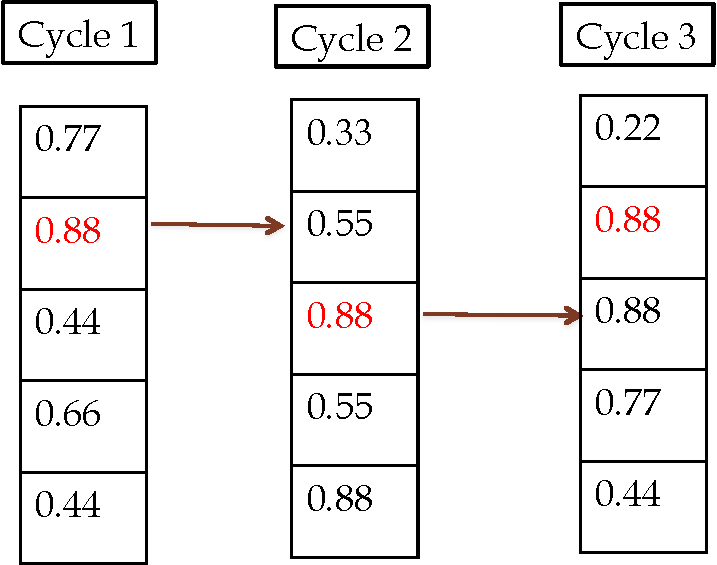
\includegraphics[width=0.5\textwidth]{figures-bharath/focus.pdf}
  \caption{Numbers in the boxes represent the compatibilities of each of the five critique strings with the target product. Simulated user selects the most compatible critique string (red) in each cycle.}
\label{fig:focus}
\end{figure}

\section{Noisy Framework}
In this scenario, the simulated user does not select the most optimal critique string during each cycle.
This kind of evaluation is similar to the evaluation procedure described in \cite{suggestion}.
Noise is introduced into the process by varying the compatibility scores of the critique strings within some threshold. 
In our experiments, we have used a noise level of 10\%, i.e, the compatiblity scores can be changed by upto +/-10\% of their actual values.
Due to the introduction of noise, the uesr makes sub-optimal choices in each cycle as seen in Figure \ref{noisy}.

\begin{figure}
  \centering
  \captionsetup{justification=centering}
    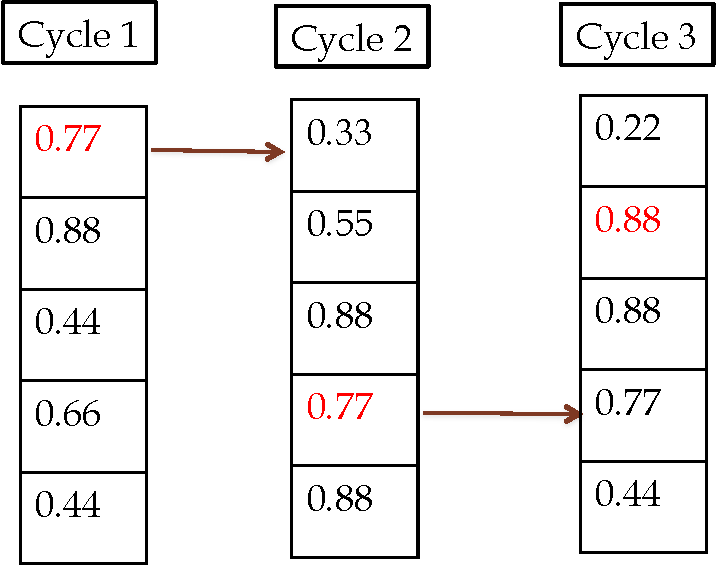
\includegraphics[width=0.5\textwidth]{figures-bharath/noisy.pdf}
  \caption{Simulated user selecting sub-optimal critique strings due to the introduction of noise}
\label{fig:noisy}
\end{figure}
